\chapter{Herramienta $\mathtt{SAT\_Solver}$}

En el presente capítulo se expondrá una herramienta para resolver el famoso problema de satisfacibilidad o más conocido como el problema $SAT$. Dicha herramienta se basará en la teoría presentada en los capítulos anteriores, mostrando así una de sus más relevantes aplicaciones. \\

Antes de tratar la herramienta, se pondrá al lector en situación dando una descripción detallada del problema de satisfacibilidad booleana; así como de su importancia, tanto para la comunidad científica internacional como para el resto de las personas.\\

Posteriormente, se describirán las tecnologías clave utilizadas en el desarrollo de la herramienta, que han dotado de estructura al proyecto además de concederle cierta robustez.\\

Finalmente, se realizará un análisis de eficiencia de la herramienta, durante el cual se detectaron ciertas ``fugas de tiempo''. Estas posibles mejoras se implementarán también dando lugar a una primera versión del \texttt{SAT-Solver}.

\newpage
\section{El problema $SAT$}

%\subsection{Definición}
Tal y como se definió en la página \pageref{def:sat}, una fórmula $F$ se dice \textit{satisfacible} si existe al menos una interpretación $i$ de $F$ que sea modelo de la fórmula. A partir de esta definición, es natural preguntarse cuándo una formula dada es satisfacible o no. Éste es el problema de la satisfacibilidad booleana o el comúnmente conocido como problema $SAT$. En definitiva consiste en saber \textit{a priori} si existe alguna forma de sustituir las variables proposicionales por $True$ o $False$, de manera que la fórmula sea verdadera. \\

Es importante destacar que para una fórmula con 10 variables, existen $2^{10} = 1024$ valoraciones a comprobar. Si a esto se suma que para que una fórmula se considere ``mínimamente interesante'' (en el mundo empresarial, por ejemplo) debe tener cientos de variables; el orden de magnitud de comprobaciones que se han de hacer es similar al número de átomos que hay en el universo. Este crecimiento tan rápido de combinaciones se debe a la complejidad exponencial intrínseca al problema de satisfacibilidad. \\

En teoría de la complejidad computacional, es considerado el problema capital de la clase de complejidad $NP$ al ser también un problema $NP$ duro ($NP$-hard), y ganándose así el estatus de problema $NP$-completo. \\

Respecto a los problemas $NP$-completos, no hay manera eficiente conocida de localizar una solución. Es decir, el tiempo requerido para resolver el problema usando cualquier algoritmo actualmente conocido aumenta muy rápidamente a medida que el tamaño del problema crece.\\

Como consecuencia, el problema de determinar si es posible resolver estos problemas de forma rápida, llamado problema $P$ versus $NP$ (¿$P=NP$?), es uno de los principales problemas sin resolver de la informática actual. Es por esto que en el año 2000, el \textit{Clay Mathematics Institute} lo declaró como el primer problema del milenio, junto a otros siete. Este título no es vano, ya que se cree que estos problemas marcarán el devenir de la comunidad científico-matemática.\\

Para comprender algo mejor la importancia del problema ¿$P=NP$? es importante conocer las consecuencias de su resolución. Si resultara que no son iguales, el impacto en la sociedad sería mínimo ya que únicamente se dejarían de buscar algoritmos de complejidad polinomial para resolver problemas de la clase $NP$.\\

Sin embargo, si se demostrase que ambas clases de complejidad son iguales, las implicaciones para la sociedad actual serían de una magnitud incomparable. Esto se debe a que la robustez de los sistemas criptográficos actuales se basan en la intratabilidad de ciertos problemas de la clase $NP$. Si éstos fueran resolubles en tiempo polinomial peligrarían todas las comunicaciones y las claves bancarias dejarían de ser seguras. Por otro lado, no todas las consecuencias son negativas ya que multitud de problemas de ámbito empresarial o social serían tratables; y por tanto, los costes se reducirían y los beneficios aumentarían.\\

Aunque, una vez vista la importancia del problema ¿$P=NP$? es natural preguntarse cómo podría resolverse. La respuesta es tan sencilla como dar un algoritmo que trabaje en tiempo polinomial en función del dato de entrada para un problema $NP$-completo, o demostrar que no existe dicho algoritmo. \\ 

El problema $NP$-completo objeto de la mayoría de estudios por parte de la comunidad científica es el problema $SAT$. Es tal su popularidad que cada año se publican multitud de nuevos algoritmos que dicen mejorar la eficiencia de resolución, y que se basan en las técnicas informáticas más innovadoras. \\

Con el objetivo de regular dicha competición, así como de identificar y promover nuevos retos relacionados con la resolución del problema $SAT$ surge la \textit{SAT Competition 2002}, enmarcada dentro del \textit{Fifth  International Symposium on the Theory and Applications of Satisfiability Testing}. Y desde ese año, de forma anual o bianual, se celebra tal competición. \\

Enmarcando el trabajo aquí presente en el contexto actual, éste pretende sentar las bases de un programa que resuelva el problema $SAT$ en un tiempo eficiente y que cumpla los estándares de dicha competición. Es por lo que a partir de este punto, la eficiencia será una máxima.\\

 Además, para poder participar en dicha competición se deben seguir un estándar. Principalmente, que la fórmula (o base de conocimiento) de entrada está escrita en un fichero de texto en forma normal conjuntiva.
 
 



%\subsection{Implicaciones}

\section{Gestión del proyecto}

\subsection{Lenguaje Haskell}

\subsubsection{Haskell Literario}

\subsection{GitHub}

\subsection{Stack}

\section{La herramienta}
A continuación, se describirán los distintos módulos de la herramienta, detallando los procesos más relevantes. Es importante destacar que los cálculos llevados a cabo por el programa se dividen principalmente en dos etapas:
\begin{enumerate}
\item Preprocesado del fichero de entrada.
\item Decisión por saturación con la regla de independencia.
\end{enumerate}

\subsection{Fichero de entrada y el formato \texttt{DIMACS}}
Previo a la descripción del formato \texttt{DIMACS} es necesaria una definición formal de qué es la forma normal conjuntiva. Con este objetivo se verán antes dos definiciones de la lógica proposicional.

\defn Un literal es una fórmula atómica o su negación. Se dice que un literal es \textit{positivo} si se trata de un átomo y \textit{negativo} si es la negación de un átomo.\\

Por ejemplo, $p_1$, $p_2$ ó $\neg p_1$ son literales.

\defn Una cláusula es una disyunción de literales. En otras palabras, es una colección finita de literales que se hace verdadera si alguno de ellos lo es. \\

Por ejemplo, $p_1 \vee p_2$ ó $p_1 \vee \neg p_2 \vee \neg p_3$ son cláusulas. Ya se está en condiciones de definir la forma normal conjuntiva.

\defn Dada una fórmula proposicional $F$ se dice que está en forma normal conjuntiva si se trata de una conjunción de cláusulas. \\

De cara al problema de satisfacibilidad es importante saber el que criterio debe cumplir una fórmula en forma normal conjuntiva para ser verdadera. Esta condición es que en todas sus cláusulas debe haber al menos un literal que sea verdadero.\\

Otra propiedad que se debe conocer sobre la forma normal conjuntiva es que dada cualquier fórmula proposicional existe otra equivalente en forma normal conjuntiva. El algoritmo \cite{apuntes} que la calcula es el siguiente:

\begin{center}
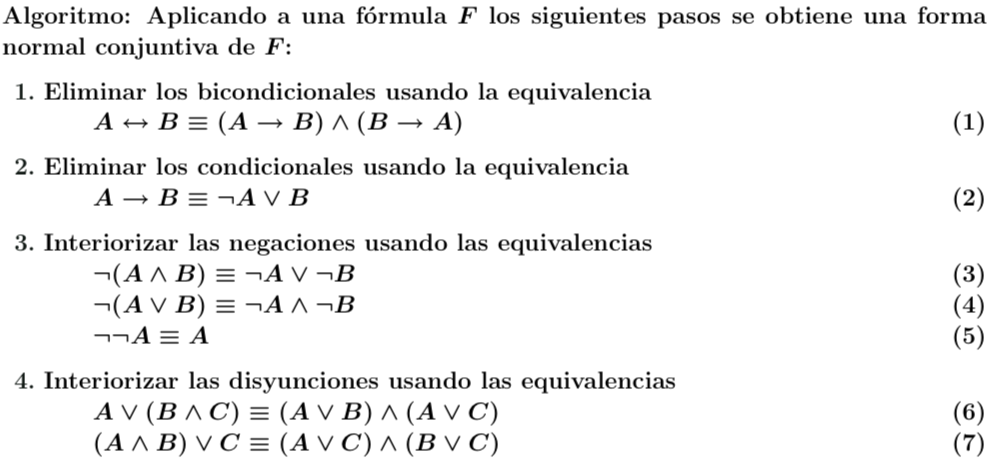
\includegraphics[scale=0.45]{imagenes/algfnc}
\end{center}

Como ya se ha comentado, se pretende presentar la herramienta a una competición, por tanto, debe cumplir ciertos requisitos para poder participar. El principal y más importante es que las instancias del problema $SAT$ que debe resolver vienen dadas en lo que se denomina el formato \texttt{DIMACS}. Un ejemplo de cómo se codificaría la fórmula $(p_1 \vee \neg p_5 \vee p_4)\wedge(\neg p_1 \vee p_5 \vee p_3 \vee p_4) \wedge (\neg p_3 \vee \neg p_4)$ en formato \texttt{DIMACS} es
\begin{table}[h]
\centering
\label{ej:dimacs}
\begin{tabular}{l}
{\Large \texttt{c} }\\\\
{\Large \texttt{c start with comments}} \\\\
{\Large \texttt{c}} \\\\
{\Large \texttt{c}}  \\\\
{\Large \texttt{p cnf 5 3}} \\\\
{\Large \texttt{1 -5 4 0}} \\\\
{\Large \texttt{-1 5 3 4 0}} \\\\
{\Large \texttt{-3 -4 0}}
\end{tabular}
\end{table}

Dicho formato es una estandarización simplificada de la forma normal conjuntiva de una fórmula. Las instancias serán archivos de texto (\texttt{.txt} o \texttt{.cnf}) con la siguiente estructura:

\begin{enumerate}
\item En primer lugar, se encuentran las líneas de comentarios. Se identifican gracias a que están encabezadas por la letra \texttt{c}. En el ejemplo, son las cuatro primeras líneas.
\item En segundo lugar, hay una línea distinguida que indica las propiedades de la fórmula como, por ejemplo, que está en forma normal conjuntiva (\texttt{cnf}). El segundo número que aparece indica cuántas variables proposicionales intervienen mientras que el segundo cuántas cláusulas.
\item Finalmente, en cada línea se encuentra codificada una cláusula distinta según las siguientes indicaciones:
\begin{itemize}
\item Cada número entero representa un literal.
\item El signo del número, positivo o negativo, indica si dicho literal es positivo o negativo, respectivamente.
\item El final de la cláusula se codifica con un 0.
\end{itemize} 
\end{enumerate}

\subsection{Preprocesado}

Las funciones que intervienen en el preprocesado tratan de transformar un archivo \texttt{.txt} ó \texttt{.cnf} en formato \texttt{DIMACS} al conjunto de polinomios que les corresponde según la función $\pi$. A continuación, se presentan estas funciones.

\entrada{Preprocesado}

\newpage
\subsection{Cálculo}

Una vez que se tiene el conjunto de polinomios basta saturar dicho conjunto usando la regla de independencia. Las funciones encargadas de realizar dicho proceso son: \texttt{omiteVariableKB} y \texttt{saturaKB}. El módulo en el que se implementarán será \texttt{Saturacion}:

\entrada{Saturacion}

\newpage
\section{Análisis de la herramienta}

\subsection{Heurísticas}